% Example questions to demonstrate answering questions in LaTeX

% THIS IS A COMMENT

% Specify document class - we're using article but there is also letter and beamer
% article is a mandatory parameter enclosed in {}
% 11pt and a4paper are optional parameters enclosed in []
\documentclass[11pt, a4paper]{article}

% Additional packages- import special commands
\usepackage{geometry} % Allows changing of page layout
\usepackage{amsmath} % Allows equations to be used
\usepackage{amssymb}
\usepackage{graphicx}
\usepackage{listings}
\usepackage{natbib}
\usepackage{enumerate}

% DOCUMENT LAYOUT
\geometry{a4paper, textwidth=6.25in, textheight=9.7in, marginparsep=7pt, marginparwidth=.6in}
\setlength\parindent{0in} % I like removing the paragraph indent

% Set title and author of document
\title{LaTeX example question answers}
\author{Michael Manansala}

% Everything between the begin and end commands will be made into the document
\begin{document}
	
	% Generate the title
	\maketitle
	
	\tableofcontents
	\pagebreak
	
	% We have a numbered list of questions- hence enumerate
	\section{Questions}
	\begin{enumerate}
		% Each item is a new number
		\item Solve the following for x:\\ % Use \\ for a new line
		% Everything in between begin and end equation is in math mode
		\begin{equation*} % Use a * to have the equation unnumbered
		(x-3)^2+4x=3x^2+7
		\end{equation*}
		\item Find the product of the following matrices A and B:\\
		\begin{equation*}
		% This is how you do a matrix
		A=\begin{pmatrix}
		3 & 4 & 2 \\
		1 & -1 & 0
		\end{pmatrix}
		B=\begin{pmatrix}
		2 & -1 \\
		4 & 0  \\
		6 & -2
		\end{pmatrix}
		\end{equation*}
		\item It is given that:\\
		\begin{equation*}
		\frac{dx}{dt}=10-4x
		\end{equation*}
		% Use $ for inline math expressions
		Find an expression for $x(t)$ and plot the value for $0\leq t\leq 5$ if $x(0)=1$.
		\item Write a function to calculate the nth Fibonacci Number using the programming language of your choice.
	\end{enumerate}
	
	\section{Answers}
	\begin{enumerate}
	    \item
	    \begin{align*} % Use align for multiple lines in an equation
	        (x-3)^2+4x&=3x^2+7\\ % & in front of = to make them line up
	        x^2-6x+9+4x&=3x^2+7\\
	        2x^2+2x-2&=0\\
	        x^2+x-1&=0\\
	        x&=\frac{-1\pm \sqrt{1^2-4\times 1\times -1}}{2}\\
	        &=\frac{-1\pm \sqrt{5}}{2}
	    \end{align*}
	    \item 
    	\begin{equation*}
        	A=\begin{pmatrix}
        		3 & 4 & 2 \\
        		1 & -1 & 0
        		\end{pmatrix}
        		B=\begin{pmatrix}
        		2 & -1 \\
        		4 & 0  \\
        		6 & -2
        	\end{pmatrix}
    	\end{equation*}
    	\begin{align*}
    	    AB&=\begin{pmatrix}
    	    3\times 2 + 4\times 0 + 2\times 6 & 
    	    3\times -1 + 4\times 0 + 2\times -2\\
    	    1\times 2 -1\times 4 + 0\times 6 &
    	    1\times -1 -1\times 0 +0\times -2\\
    	    \end{pmatrix}\\
    	    &=\begin{pmatrix}
    	    34 & -7\\
    	    -2 & -1
    	    \end{pmatrix}
    	\end{align*}
    	\item \begin{align*}
    	    \frac{dx}{dt} &= 10-4x\\
    	    \frac{dx}{10-4x} &= dt\\
    	    \int{\frac{dx}{10-4x}} &= \int{dt}\\
    	    -\frac{1}{4}\ln{(10-4x)} &= t+C\\
    	    \ln{10-4x} &= -4(t+C)\\
    	    10-4x &= e^{-4(t+C)}\\
    	    4x &= 10-e^{-4(t+C)}\\
    	    x &= 2.5-\frac{1}{4}e^{-4(t+C)}\\
    	    &= 2.5 - Ae^{-4t}
    	\end{align*}
    	When $t=0$, $x=1$.
    	\begin{equation*}
    	    1 = 2.5 - Ae^0 = 2.5 - A
    	\end{equation*}
    	\begin{equation*}
    	    \therefore A = 1.5
    	\end{equation*}
    	\begin{equation*}
    	    \therefore x = 2.5 - 1.5e^{-4t}
    	\end{equation*}
    	This is shown in figure \ref{fig:xplot}:\\
    	\begin{figure}[htb]
    	    \centering
        	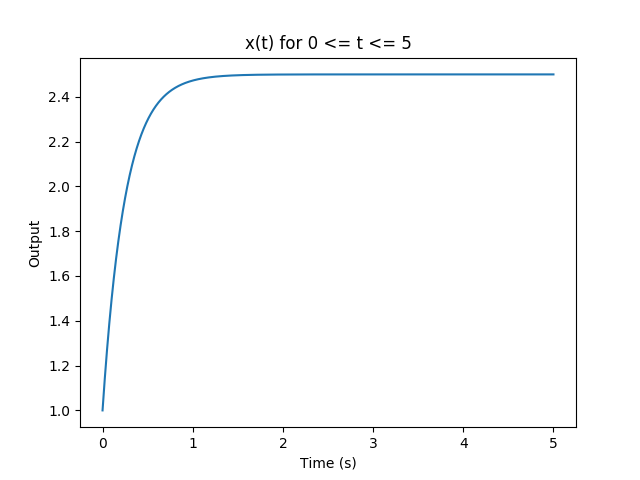
\includegraphics[width=0.8\columnwidth]{xplot.png}
    	    \caption{Plot of x}
    	    \label{fig:xplot}
    	\end{figure}
    	\pagebreak
    	\item The Fibonacci sequence is defined by $F_0 = 0$, $F_1 = 1$ and $F_n = F_{n-1} + F_{n-2}$ (\cite{bib:fib}):
    	\begin{lstlisting}
def fib(n):
    if n <= 0:
        return 0
    elif n == 1:
        return 1
    else:
        return fib(n-1) + fib(n-2)
    	\end{lstlisting}
	\end{enumerate}
	
	\section{Random Features}
	Things to do today:
	\begin{itemize}
	    \item Run workshop
	    \item Eat lunch
	    \item Finish assignment
	\end{itemize}
	
	\bibliographystyle{agsm}
	\bibliography{references}
	
\end{document}